\graphicspath{{img/chapter_2/}}



\chapter{A Primer on Compact Objects}
\label{chapter:compactobjects}

% \begin{synopsis}
% Introduce COs, formation, structure etc...  
% \end{synopsis}
%%%%%%%%%%%%%%%%%%%%%%%%%%%%%%%%%%%%%
%%%%%%%%%%%%%%%%%%%%%%%%%%%%%%%%%%%%%
%%%%%%%%%%%%%%%%%%%%%%%%%%%%%%%%%%%%%

Within the cores of stars exists a delicate balance between the gravitational force of its mass wanting to collapse in on itself, and the outward pressure generated by thermonuclear fusion of light elements. This fusion process begins with the burning of hydrogen to form helium. Eventually, the hydrogen is depleted, allowing gravity to temporarily overcome the outward pressure leading to the core contracting. As this occurs, the gravitational potential energy is converted to thermal energy and the core eventually becomes hot enough to facilitate helium burning. 

This cycle continues as heavier and heavier elements are formed within the ever-increasingly hot stellar core.
If the star is heavy enough, iron will eventually be formed from the burning of silicon. As the fusion of iron nuclei is an endothermic process, it will not occur spontaneously. Whatever the mass of the star, eventually it will no longer be able to support the fusion of these heavier elements. Without a sufficient fuel source, the core will collapse under its own gravity leading to the death of the star.  

What comes after this depends on the mass of the progenitor stars. Very light stars, $\lesssim 0.5 \Msun$, have lifetimes much longer than the age of the universe, and so are uninteresting to our current discussion. Moderately heavy stars, $1\Msun\lesssim \Mstar \lesssim 8\Msun$, will continue burning fuel until the outer layers of the star are dispersed as it expands, leaving a carbon-oxygen (CO) core. The core will begin to collapse until the Fermi degeneracy of the ultrarelativistic electrons is great enough to reestablish equilibrium, resulting in a White Dwarf (WD).

Heavy stars, $\gtrsim 8\Msun$, spectacularly end their lives in a type-II supernova event. This occurs when the core of the star exceeds the Chandrashekhar mass of $1.4\Msun$, which cannot be supported by electron degeneracy pressure. The core itself will then collapse, leading to a shockwave that ejects the majority of the mass of the star. All that will remain is an extremely dense core supported by neutron degeneracy pressure, a Neutron Star (NS). If the star was so massive that the gravitational forces overcome even the neutron degeneracy pressure, then the core collapses into a black hole. 

These three stellar corpses (white dwarfs, neutron stars, and black holes) are collectively known as compact objects, as they have masses similar to or larger than our Sun, compressed into much smaller bodies with significantly larger surface gravities. These objects do not have a source of fuel, and spend the rest of their lives cooling down. For the remainder of this thesis, we will only be interested in white dwarfs and neutron stars and refer to these collectively as compact objects, excluding black holes from this term. 

This chapter is dedicated to discussing the structure and composition of these objects\footnote{As this work is written by a particle physicist, I wish to apologise to my astrophysics colleagues for what is to come.}.


%%%%%%%%%%%%%%%%%%%%%%%%%%%%%%%%%%%%%
%%%%%%%%%%%%%%%%%%%%%%%%%%%%%%%%%%%%%
%%%%%%%%%%%%%%%%%%%%%%%%%%%%%%%%%%%%%
\section{Structure Equations from General Relativity}
%%%%%%%%%%%%%%%%%%%%%%%%%%%%%%%%%%%%%
%%%%%%%%%%%%%%%%%%%%%%%%%%%%%%%%%%%%%

The highly dense matter comprising neutron stars and white dwarfs leads to extremely strong gravitational fields being produced by the stars. As such, modeling the structure of these objects falls into the domain of General Relativity (GR). Here we review the structure of static, spherically symmetric stars. 

The assumption that the mass distribution of the star is spherically symmetric leads to the metric taking the form
\begin{equation}
    ds^2 = -d\tau^2 = -B(r) dt^2 + A(r) dr^2 + r^2 d\Omega^2,
\end{equation}
with $d\tau$ the proper time interval, and $A(r),\;B(r)$ are functions only of the radial coordinate and are often written as 
\begin{equation}
    A(r) = e^{2\Lambda(r)},\quad B(r) = e^{2\Phi(r)}.
\end{equation}
These functions are subject to the condition that at distances far from the star space-time becomes flat, leading to the boundary conditions 
\begin{equation}
    \lim_{r\rightarrow \infty} A(r) = \lim_{r\rightarrow \infty} B(r)  = 1.
\end{equation}

The matter that comprises the star is modeled as a perfect fluid, meaning we are neglecting any shear stresses and energy transport within the star. Such a fluid is described by its pressure $P(r)$, density $\rho(r)$, and number density, $n(r)$, as well as the 4-velocity of the fluid $u^\mu(r)$. Being a static fluid, the only non-zero component of this velocity is the time component, which is fixed through $g_{\mu\nu}u^\mu u^\nu = -1$ to be $u^t = 1/\sqrt{B(r)}$.
These quantities are then used to construct the stress-energy tensor for the star, which takes the form
\begin{equation}
    T^{\mu\nu} = (\rho + P)u^\mu u^\nu + P g^{\mu\nu}.
\end{equation}
The microphysics underlying the matter interactions are encoded in an equation of state (EoS) that relates the various thermodynamic quantities. This is typically given by expressing the pressure as a function of the density, $P(\rho)$. It is often more convienient to parameterise the EoS by the number density of baryons, $n_b$, and the entropy per baryon, $s$, such that 
\begin{equation}
    P=P(n, s), \quad \rho = \rho(n, s).
\end{equation}
The dependence on $s$ turns out to be trivial in most scenarios involving compact objects, such as those considered here. The pressure in these stars arises from the degeneracy of the nucleons in NSs or the electrons in WDs, rather than from the thermal motion of the constituents that will be frozen out at low temperatures. This is the case for temperatures much lower than the Fermi energy of the system, with typical values of $E_F \sim 10\MeV$ in NSs or $\sim 1 \MeV$ in WDs, corresponding to temperatures of $T_\star\sim 10^{11}\K$ and $\sim 10^{10}\K$ respectively. As these stars are expected to cool well below these temperatures quickly after formation, the entropy can be taken to be zero throughout the star. This allows us to reduce the two-parameter EoS to a simpler one-parameter one,
\begin{equation}
    P=P(n_b, s = 0) = P(n_b), \quad \rho = \rho(n_b, s=0) = \rho(n_b).\label{eq:1_param_EoS}
\end{equation} 


The structure of the star is therefore determined by the quantities $A(r)$, $B(r)$, $P(r)$, $\rho(r)$, and $n_b(r)$. This system is determined by applying the Einstein field equations, $G^{\mu\nu} = 8\pi T^{\mu\nu}$, together with the conservation of energy-momentum, $T^{\mu\nu}_{\quad;\nu}=0$, the EoS relations Eqs.~\ref{eq:1_param_EoS}, and the appropriate boundary conditions. The structure equations that come out of this analysis were first discovered concurrently by Tolman~\cite{Tolman:1939jz_StaticSolutionsEinstein} and by Oppenheimer and Volkoff~\cite{Oppenheimer:1939ne_MassiveNeutronCores}, and so are known as the TOV equations. They take the form
\begin{align}
    \frac{dP}{dr} &= -\rho(r) c^2  \left[ 1 + \frac{P(r)}{\rho(r) c^2} \right]\frac{d\Phi}{dr},\label{eq:TOV_1}\\
    \frac{d\Phi}{dr} & = \frac{G M(r)}{c^2 r^2} \left[ 1 + \frac{4\pi r^3 P(r)}{M(r)c^2} \right] \left[ 1 - \frac{2 G M(r)}{c^2 r}\right]^{-1}\label{eq:TOV_2},\\
    \frac{dB}{dr} & = 2B(r) \frac{d\Phi}{dr},\label{eq:TOV_3}
\end{align}
where $M(r)$ is related to the metric factor $A(r)$ through
\begin{equation}
    A(r) = \left[ 1 - \frac{G M(r)}{c^2 r} \right]^{-1},
\end{equation}
and is interpreted as the mass contained within a radius $r$. It obeys the mass equation 
\begin{equation}
    \frac{dM}{dr} = 4\pi r^2 \rho(r),\quad M(0) = 0,
    \label{eq:mass_equation_TOV}
\end{equation}
that arises from the $\mu = \nu = 0$ component of the Einstein field equiations. 
These equations are the general relativistic versions of the hydrostatic equilibrium equations of regular stellar structure, with Eq.~\ref{eq:TOV_1} reducing to the familiar 
\begin{equation}
    \frac{dP}{dr} = -\frac{GM(r)}{r^2}\rho(r),
\end{equation}
in the Newtonian limit, $GM(r)/c^2 r \ll 1$.

The radius of the star, $\Rstar$, is identified as the point at which the pressure and density vanish, $P(\Rstar) = \rho(\Rstar) = 0$. In the region outside the star, $r>\Rstar$, the total mass remains constant at the total mass of the star, $M(r \geq  \Rstar) = \Mstar$, and so the only non-trivial structure functions are the metric factors. Solving Eq.~\ref{eq:TOV_3} with $P(r)=0$ and constant $M(r)$ for $B(r)$ becomes elementary while the result for $A(r)$ is trivial, leaving us with
\begin{equation}
    A(r) = \left[ 1 - \frac{G \Mstar}{c^2 r} \right]^{-1}, \quad B(r) = 1 - \frac{G \Mstar}{c^2 r} ,\quad\mathrm{for}\;r > \Rstar,
\end{equation}
and the metric reduces to the familiar Schwarzschild metric outside the star. 
Continuity of the metric at $r= \Rstar$ enforces a second boundary condition for $B(r)$,
\begin{equation}
    B(\Rstar) = 1 - \frac{G \Mstar}{c^2 \Rstar}.
    \label{eq:B_boundary_condition}
\end{equation}

The final boundary condition required is the central pressure $P(0) = P_c$, or equivalently the central density/baryon number density. This is the only free parameter in the system and hence, for a given EoS, uniquely determines the stellar structure. All stars generated by an EoS can therefore be represented as a one-parameter sequence, typically represented as the mass-radius relation for the model. 

Given all the above, we can write a simple recipe for constructing a model of a compact object:
\begin{enumerate}
    \item Select an EoS to describe the constituent matter.
    \item Specify the central pressure of the star, $P_c$.
    \item Integrate the coupled system of differential equations \ref{eq:TOV_1}, \ref{eq:TOV_2}, \ref{eq:mass_equation_TOV} from the centre of the star outward until the pressure vanishes.
    \item Use the boundary condition Eq.~\ref{eq:B_boundary_condition} to normalise the metric function $B(r)$. 
\end{enumerate}
In general, additional quantities will be present in the EoS, such as chemical potentials or the speed of sound, that may be subject to additional constraints. These quantities will need to be calculated at each step of the integration alongside the other EoS quantities. 

%%%%%%%%%%%%%%%%%%%%%%%%%%%%%%%%%%%%%
%%%%%%%%%%%%%%%%%%%%%%%%%%%%%%%%%%%%%
%%%%%%%%%%%%%%%%%%%%%%%%%%%%%%%%%%%%%
\section{White Dwarfs}
%%%%%%%%%%%%%%%%%%%%%%%%%%%%%%%%%%%%%
%%%%%%%%%%%%%%%%%%%%%%%%%%%%%%%%%%%%%
%%%%%%%%%%%%%%%%%%%%%%%%%%%%%%%%%%%%%

The fate of main sequence stars of mass below $\Mstar \lesssim 8 - 10 \Msun$ is to end their life cycles as a white dwarf. Consequently, these compact stellar remnants, which are supported against gravitational collapse by electron degeneracy pressure, are the most abundant stars in the Galaxy ($\gtrsim 90\%$). They are born at very high temperatures and cool down over billions of years. Observations of the coldest WDs therefore contain information on the star formation history of the Galaxy.

The vast majority of observed WDs are composed primarily of carbon and oxygen, plus small traces of elements heavier than helium. 
At the extremely high densities found in WDs $\sim10^6-10^{10}\g\cm^{-3}$, electrons are strongly degenerate and determine the WD equation of state (EoS) and internal structure.  The stellar core resembles a Coulomb lattice of ions surrounded by degenerate electrons, which implies that the WD core is isothermal and a very good thermal conductor. 
The degenerate core is enclosed by a thin envelope that accounts for $\lesssim 1\%$  of the total mass~\cite{Fontaine_apr_Potentialwhitedwarf}. 

The outer layers form an atmosphere that is rich in lighter elements such as hydrogen or helium, where the exact composition depends on the evolution of the WD progenitor and changes as the WD cools. 
This atmosphere is non-degenerate and extremely opaque to radiation, with an EoS that is subject to finite temperature effects. 

In the limit of zero temperature, the simplest way to obtain the WD EoS is to assume an ideal Fermi gas of degenerate electrons, for a WD that is primarily composed of a single element. Corrections to the non-interacting electron picture were introduced early by Salpeter~\cite{Salpeter:1961zz_nov_Energypressurezerotemperature}. By introducing the Wigner-Seitz (WS) cell approximation and assuming point-like nuclei, Salpeter obtained an analytical EoS that accounts for interactions between electrons and ions as well as other Coulomb corrections. These corrections, in general, depend on the chemical composition of the star. 

More recently, it has been shown that the treatment of matter at high pressures presented by Feynman, Metropolis and Teller~\cite{Feynman:1949zz_Equationsstateelements} can be extended to consistently take into account weak interactions and relativistic effects \cite{Rotondo:2009cr_RelativisticThomasFermitreatment,Rotondo:2011zz_RelativisticFeynmanMetropolisTellertheory}, and incorporates Coulomb corrections in a more natural manner than the Salpeter EoS. The resulting Feynman-Metropolis-Teller (FMT) EoS is obtained by considering a relativistic Thomas-Fermi model within Wigner-Seitz cells of radius $R_{\mathrm WS}$. 
For degenerate, relativistic, electrons, the equilibrium condition is that the Fermi energy, $E_e^F$, is constant within the cell,
\begin{equation}\label{eq:rel_equil}
E_e^F=\sqrt{(p_e^F)^2+m_e^2}-m_e-eV(r) = \rm{constant},
\end{equation}
where $V(r)$ is the Coulomb potential inside the cell, $p_e^F$ is the electron Fermi momentum, $m_e$ is the electron mass and $e$ is the electric charge. To obtain an integrable solution for the energy density near the origin, it is necessary to introduce a finite size for the nucleus, with radius $ R_c = \Delta\lambda_{\pi} Z^{1/3}$, 
where $\lambda_\pi$ is the pion Compton wavelength, $\Delta \approx (r_0 /\lambda_\pi)(A/Z)^{1/3}$, $Z$ is the proton number, $A$ is the atomic mass, and $r_0$ is an empirical constant $\sim 1.2\;\text{fm}$. The proton and electron number densities inside the cell are then given by
\begin{align}
    n_p &=  \frac{(p^F_p)^3}{3\pi^2} =\frac{3Z}{4\pi R_c^3}\theta( R_c - r ) = \frac{3}{4\pi} \left( \frac{1}{\Delta \lambda_\pi} \right)^3 \theta(R_c -r), \label{eq:prot_dens_FMT}\\
    n_e &= \frac{(p^F_e)^3}{3\pi^2} = \frac{1}{3\pi^2}\left[ \hat{V}^2(r) + 2m_e \hat{V}(r)\right]^{3/2},\label{eq:elec_dens_FMT}\\
    \hat{V}(r) &= eV(r) + E_e^F. \label{eq:vhat}
\end{align}
Using these expressions in the Poisson equation for the Coulomb potential results in the relativistic Thomas-Fermi equation
\begin{equation}
    \frac{1}{3x}\frac{d^2\beta}{dx^2} = -\frac{\alpha}{\Delta^3}\theta(x_c -x) + \frac{4\alpha}{9\pi}\left[ \frac{\beta^2(x)}{x^2} + 2\frac{m_e}{m_\pi}\frac{\beta(x)}{x}\right]^{3/2},\label{eq:FMT_DE}
\end{equation}
which is written in terms of the dimensionless quantities $x = r/\lambda_\pi$ and $\beta(r) = r\hat{V}(r)$, such that $x_c = R_c/\lambda_\pi$ and $x_{\mathrm WS} = R_{\mathrm WS}/\lambda_\pi$, and $\alpha$ is the fine structure constant.
The requirement of global charge neutrality imposes the conditions $dV/dr |_{r=R_{\mathrm WS}} =0$ and $V(R_{\mathrm WS}) = 0$, which translate to the boundary conditions
\begin{equation}
    \beta(0) = 0, \qquad
    \left. \frac{d\beta}{dx}\right|_{x_{\mathrm WS}} = \frac{\beta(x_{\mathrm WS})}{x_{\mathrm WS}}. \label{eq:TF_bc}
\end{equation}

By solving these equations, we can obtain the relevant thermodynamic quantities, namely the electron and proton number densities, electron chemical potential, and the energy and pressure of the cell. The electron chemical potential is obtained by evaluating Eq.~\ref{eq:rel_equil} at the cell radius, noting that the Coulomb potential must vanish there, which results in the usual expression
\begin{equation}
    \mu_{F,e} = \sqrt{(p_e^F)^2+m_e^2}-m_e.\label{eq:mufe}
\end{equation}
The energy and pressure of the cell can then be obtained following the analysis presented in~ref.~\cite{Rotondo:2011zz_RelativisticFeynmanMetropolisTellertheory}. The cell energy gains contributions from the nuclear mass, electron kinetic energy, and Coulomb interactions, such that
\begin{align}
    E_\mathrm{tot} & = M_N + E_k + E_C,\\
    E_k & = \int_0^{R_{\mathrm WS}}4\pi r^2 (\mathcal{E}_e(r) - m_e n_e(r))\;dr,\\
    E_C & = \frac{1}{2}\int_{R_c}^{R_{\mathrm WS}}4\pi r^2 e(n_p(r) - n_e(r))V(r)\;dr,
\end{align}
where 
\begin{equation}
    \mathcal{E}_e(r) = \frac{1}{\pi^2}\int_0^{p_e^F}p^2\sqrt{p^2 + m_e^2}\;dp,
\end{equation}
is the electron energy density, and  $M_N$ is the mass of the nucleus. The only contribution to the internal cell pressure comes from the electrons,
\begin{equation}
    P_e(r) = \frac{1}{3\pi^2}\int_0^{p_e^F}\frac{p^4}{\sqrt{p^2+m_e^2}}\;dp,
\end{equation}
with the total pressure of the cell being $P_\mathrm{tot} = P_e(R_{\mathrm WS})$.
Finally, the EoS is then obtained by solving Eq.~\ref{eq:FMT_DE} for various cell radii, yielding a relation between $E_\mathrm{tot}$ and $P_\mathrm{tot}$ parameterised by the radius of the Wigner-Seitz cell. 


\begin{table}[t]
  \centering
    \begin{tabular}{|l|l|l|l|l|} % <-- Changed to S here.
    \hline
      \textbf{EoS} & \textbf{WD}$_\mathbf{1}$  & \textbf{WD}$_\mathbf{2}$&\textbf{WD}$_\mathbf{3}$ &\textbf{WD}$_\mathbf{4}$\\
      \hline
     $\rho_c\,[\g\cm^{-3}]$ &  $1.47\times 10^{6}$ & $3.84\times 10^{7} $ & $3.13\times 10^{8}$ & $2.31\times 10^{10}$\\
     $\Mstar\,[M_\odot]$ & $0.440$ &  $1.000 $ & $1.252$ & $1.384$\\
     $\Rstar\,[\km]$ & $9.39\times 10^{3}$ &  $5.38\times 10^{3}$ & $3.29\times 10^3$ & $1.25\times 10^3$\\
     $\vesc(\Rstar) \, [\km/\s]$ & $3.72\times 10^{3}$ & $7.03\times 10^{3}$ & $1.01\times 10^{4}$ & $1.71\times 10^{4}$ \\
      \hline
    \end{tabular}
  \caption{Four configurations for white dwarfs composed of carbon, with an FMT EoS. Shown are the central densities, $\rho_c$, stellar mass $\Mstar$ and radius $\Rstar$, and escape velocity at the edge of the WD, $\vesc$. }
    \label{tab:WDs}
\end{table}
 


Different WD configurations can be obtained, assuming a non-rotating spherically symmetric star, by solving the
Tolman-Oppenheimer-Volkoff (TOV) equations~\cite{Tolman:1939jz_StaticSolutionsEinstein,Oppenheimer:1939ne_MassiveNeutronCores} coupled to the FMT EoS with different initial conditions for the pressure at the centre of the star. In Fig.~\ref{fig:WDradprofs} we show radial profiles for $n_e$ (top left), $\muFe$ (top right), and escape velocity $\vesc$ (bottom) for the carbon WDs in Table~\ref{tab:WDs}. Note that the difference in radius between the lightest and heaviest WD in Table~\ref{tab:WDs} spans almost one order of magnitude, while the electron number densities in the core can vary up to 4 orders of magnitude (see top left panel). As expected, electrons are more degenerate in more compact WDs and become relativistic (see top right panel). The escape velocity can reach ${\mathcal{O}}(0.1\,c)$ at the interior of the most compact WDs, while for very low mass WDs 
it can be as low as $\sim0.003\,c$. 

\begin{figure}[!t]
    \centering
    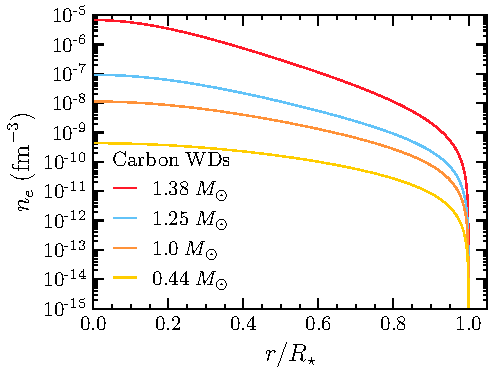
\includegraphics[width = 0.495\textwidth]{ne_prof.pdf}  
    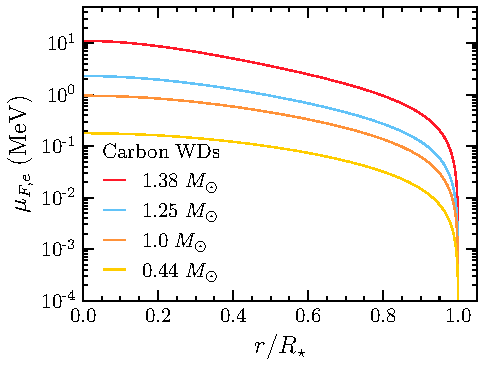
\includegraphics[width = 0.495\textwidth]{muFe_prof.pdf}  
    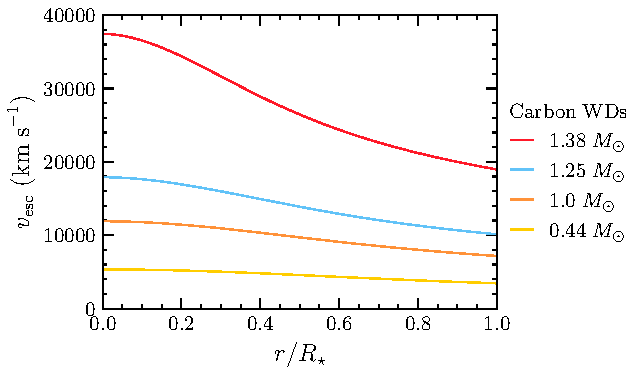
\includegraphics[width = 0.67\textwidth]{vesc_prof.pdf}
    \caption{Electron number density (top left), chemical potential (top right) and escape velocity (bottom) radial profiles for the carbon WDs with FMT EoS in Table~\ref{tab:WDs}. The radial distance of each profile has been normalised to the radius of the star.}
    \label{fig:WDradprofs}
\end{figure}

\fixMV{Discuss finite T corrections}
The mass-radius relations obtained from a zero-temperature EoS begin to deviate from observations for low-mass WDs. To address this discrepancy, finite temperature effects can be introduced to the EoS~\cite{deCarvalho:2013rea_Relativisticfeynmanmetropolistellertreatment}. When calculating the effects for carbon WDs with core temperatures $\Tstar=10^6-10^7   $K, we find that the chemical potential is smaller by only $\sim16\%$, and the number density by $\sim~35\%$.
As we shall focus on old WDs, we shall assume $\Tstar=10^5\K$, for which the zero-temperature regime holds. Note that finite temperature effects on the EoS may be more pronounced for light WDs composed of helium~\cite{deCarvalho:2013rea_Relativisticfeynmanmetropolistellertreatment}. 

%%%%%%%%%%%%%%%%%%%%%%%%%%%%%%%%%%%%%
%%%%%%%%%%%%%%%%%%%%%%%%%%%%%%%%%%%%%
\subsection{Observational Status}
%%%%%%%%%%%%%%%%%%%%%%%%%%%%%%%%%%%%%
%%%%%%%%%%%%%%%%%%%%%%%%%%%%%%%%%%%%%

%%%%%%%%%%%%%%%%%%%%%%%%%%%%%%%%%%%%%
%%%%%%%%%%%%%%%%%%%%%%%%%%%%%%%%%%%%%
%%%%%%%%%%%%%%%%%%%%%%%%%%%%%%%%%%%%%
\section{Neutron Stars}
%%%%%%%%%%%%%%%%%%%%%%%%%%%%%%%%%%%%%
%%%%%%%%%%%%%%%%%%%%%%%%%%%%%%%%%%%%%
%%%%%%%%%%%%%%%%%%%%%%%%%%%%%%%%%%%%%

Beta Equlibrium

%%%%%%%%%%%%%%%%%%%%%%%%%%%%%%%%%%%%%
%%%%%%%%%%%%%%%%%%%%%%%%%%%%%%%%%%%%%
\subsection{Observational Status}
%%%%%%%%%%%%%%%%%%%%%%%%%%%%%%%%%%%%%
%%%%%%%%%%%%%%%%%%%%%%%%%%%%%%%%%%%%%

